\documentclass[12pt, letterpaper]{article}
\usepackage{color}
\usepackage{parskip}
\usepackage{amsmath}
\usepackage{amssymb}
\usepackage{gensymb}
\usepackage{graphicx}
\usepackage{listings}
\usepackage{geometry}
\usepackage{setspace}
\usepackage{enumitem}
\usepackage{algorithm}
\usepackage{subcaption}
\usepackage{anyfontsize}
\usepackage{indentfirst}
\usepackage{algorithmic}
\usepackage[utf8]{inputenc}
\usepackage[american]{babel}
\usepackage[babel]{csquotes}
\usepackage[style=phys,
            articletitle=false,
            biblabel=brackets,
            chaptertitle=false,
            pageranges=false]{biblatex}

\addbibresource{IA.bib}
\defbibheading{bibliography}{\section{Bibliography}}
\bibliography{IA}

\geometry{letterpaper, portrait, margin=1in}
\graphicspath{{./imgs/}}

\newcommand{\sorta}[1]{`#1'}
\newcommand{\poses}[1]{#1's}

\definecolor{codegray}{rgb}{0.2,0.2,0.2}
\definecolor{codepurple}{rgb}{0.58,0,0.82}
\definecolor{backcolor}{rgb}{0.95,0.95,0.92}

\lstdefinestyle{scheme}
  {backgroundcolor=\color{backcolor},
  commentstyle=\color{blue},
  keywordstyle=\color{magenta},
  numberstyle=\tiny\color{codegray},
  stringstyle=\color{codepurple},
  basicstyle=\footnotesize\ttfamily,
  morekeywords={*},
  breakatwhitespace=false,
  breaklines=true,
  captionpos=t,
  keepspaces=true,
  numbers=left,
  numbersep=5pt,
  showspaces=false,
  showstringspaces=false,
  showtabs=false,
  tabsize=2,
  title=\lstname,
  language=Python
}

\lstset{style=scheme}

\title{Using Computer Simulations to Test the Viability of a Spring Powered Launcher}
\author{Simon Abrelat}
\date{May 2019}

\begin{document}
\large
\doublespace{}
\parindent=0.5in

{\fontsize{12}{14.4}
  {\singlespace
    \pagenumbering{gobble}
    \maketitle
    \begin{center}
    002129-0004 \\
    \vspace{4mm}
    IB Physics HL IA \\
    \vspace{4mm}
    Words:  \\ % words
    \end{center}
  }
}	


\newpage
\tableofcontents
\pagenumbering{arabic}
\newpage

\section{Introduction} \label{sec:Introduction}
In the design process, there needs to be a way to vet interesting and alternative ideas. On my robotics team,
one way to do this with computer simulations. To scale a 13 inch (33 cm) vertical step the idea of a spring
powered launch was brought up, so its efficacy had to be determined. The idea was to angle the robot and have
a pogo-inspired launcher spring out from the back of the robot. The goal of this simulation is to
approximately test if this design possible, and, if its theoretically possible, if the materials are
reasonable.

\subsection{Design Constraints} \label{sec:DesignConstraints}
This robot is designed for the FIRST Robotics Competition (FRC), so there are a lot of rules that inform what
is possible. There must be a padded bumper that is no more than 3 inch (7.6 cm) off of the ground. This
greatly limits the angle we are able to tilt the robot, for this simulation a max angle of $50\degree$. There
is also a weight limit of 150 lbs (69 kg). This weight will be used for the simulation to prove that the
design can work in a variety of situations and is more consistent. There are space constraints, but they are
not being factored in for this simulation since those are more design specific implementation details over
physic constraints.

\section{Simulation} \label{Simulation}
This simulation has 2 sections: acceleration and flight. The acceleration uses the spring to force the robot
up. The flight is the projectile motion of the robot in the air. Given the design constraints
(Section~\ref{sec:DesignConstraints}), there are simulation constants like a weight of 69 kg and angle of 
$50\degree$.

\subsection{Spring Acceleration} \label{sec:SpringAcc}
Acceleration has to be calculated from the force of the spring. The spring force is approximated by Hooke's
Law (\ref{eq:hooke}). Hooke's Law states the force is proportional to the distance of compression of the
spring. The slope of this proportion would then be the spring constant which is measured in Newtons per
meter. So for each meter compressed the spring exerts that many Newtons of force. 

\begin{singlespace}
  \begin{equation}
    \label{eq:hooke}
    F_s = -kx
  \end{equation}
  \begin{small}
    \begin{itemize}[label=]
      \item $F_s$: Force of the spring, $N$
      \item $k$: Spring constant, $\dfrac{N}{m}$
      \item $x$: The displacement of the spring, $m$
    \end{itemize}
  \end{small}
\end{singlespace}

The force is then used to describe the acceleration using \poses{Newton} second law (\ref{eq:n2}). The
vertical acceleration from the spring is then reduced by the force due to gravity giving the net acceleration
on the object. This net force is described by equation \ref{eq:netforce}.

\begin{singlespace}
  \begin{equation}
    \label{eq:n2}
    \vec{F} = m \vec{a}
  \end{equation}
  \begin{small}
    \begin{itemize}[label=]
      \item $\vec{F}$: Force vector, $N$
      \item $m$: Mass, $kg$
      \item $\vec{a}$: Acceleration vector, $\dfrac{m}{s^2}$
    \end{itemize}
  \end{small}
  \begin{equation}
    \label{eq:netforce}
    m a = -k x - m g
  \end{equation}
  \begin{small}
    \begin{itemize}[label=]
      \item $a$: Net acceleration, $\dfrac{m}{s^2}$
      \item $k$: Spring constant, $\dfrac{N}{m}$
      \item $m$: Mass, $kg$
      \item $g$: Acceleration due to gravity, $9.81 \dfrac{m}{s^2}$
    \end{itemize}
  \end{small}
\end{singlespace}

The acceleration of the object decreases the distance which then decreases the force and the net force is
decreased by gravity (\ref{eq:diffAcc}), full derivation in Equation~\ref{eq:derivation}. This generates a 
cyclical decay in force. For this simulation, this second degree differential equation would be approximated 
using Euler's method.

\begin{equation}
  \label{eq:diffAcc}
  \ddot{x} = \frac{-kx}{m} -g
\end{equation}

Equation~\ref{eq:diffAcc} is calculated by solving the equation in repeating small steps. For this, the 
equation gives you acceleration given a position, the acceleration determines the velocity which moves the 
position as described in Algorithm~\ref{alg:accSolver}.


\begin{algorithm}
\caption{Acceleration Solver}
\begin{algorithmic} 
\label{alg:accSolver}
\REQUIRE $v, a = 0$
\REQUIRE $g = 9.81$
\REQUIRE $t = 0.001$
\REQUIRE $x =$ starting displacement
\REQUIRE $k =$ spring constant
\WHILE{$x \geq 0$}
\STATE $a \leftarrow \dfrac{-kx}{m} - g$
\STATE $v \leftarrow v + a * \Delta t$
\STATE $x \leftarrow x + v * \Delta t$
\ENDWHILE
\end{algorithmic}
\end{algorithm}

\subsection{Projection Motion} \label{sec:ProjectileMotion}
There are two different ways to simulate the projectile motion: iterative and formulaic. The iterative method
uses a series of differential equations following the assumptions of projectile motion. The assumptions are
the gravity pushes down on the vertical axis and there is no force opposing horizontal motion.

\begin{singlespace}
  \begin{equation}
    \begin{split}
      &\dot{x} = \cos(\theta) v \\
      &\dot{y} = v_v \\
      &\dot{v_v} = g \\
    \end{split}
  \end{equation}
  \begin{small}
    \begin{itemize}[label=]
      \item $\theta$: initial angle
      \item $v$: initial velocity
      \item $v_v$: vertical velocity
    \end{itemize}
  \end{small}
\end{singlespace}

Much like the \poses{Hooke} equation solver, Algorithm~\ref{alg:accSolver}, the approximation for this motion
uses \poses{Euler} method to iterate through time and accumulate toward the answer, as shown in
Algorithm~\ref{alg:projSolver}. \poses{Euler} method is a way to solve differential or integral equations by
summing the output of your equation by some arbitrarily small $\Delta t$, this gets the \sorta{area under
the curve}. Then the algorithm iterates the position using the velocity and the vertical component of the 
velocity by the acceleration from gravity.

\begin{algorithm}
\caption{Projectile Motion Approximation}
\begin{algorithmic} 
\label{alg:projSolver}
\REQUIRE $g = -9.81$
\REQUIRE $t = 0.001$
\REQUIRE $v =$ starting velocity
\REQUIRE $\theta =$ starting angle
\REQUIRE $v_v = \sin(\theta) v$
\WHILE{$x \geq 0$}
\STATE $y \leftarrow  y + \cos(\theta) v * \Delta t$
\STATE $v_v \leftarrow  v_v + g * \Delta t$
\STATE $x \leftarrow  y + v_v * \Delta t$
\ENDWHILE
\end{algorithmic}
\end{algorithm}

This method is similar to the prior method used in Algorithm~\ref{alg:accSolver}. The problem with it is that
not only the value accumulates but any error. The benefit is greater control and visibility into
the program, as well as the more intuitive explanation because you need to describe that happens in a single
moment. In more complex simulations, this method is better because it allows for drag and rotational forces,
but for this proof-of-concept those are not required. That means that we should use the formulaic approach.
The problem with the formulaic approach is with the vertical step which cuts off the motion of the object
sooner than expecting and trying to get close to an optimal angle is difficult. This means you need additions
to the general projectile motion equations, and it looses some of its generality in the process. Another
problem is that if the pogo does not behave as the equations predict, invalid answers are returned. In normal
projectile motion, the hight is governed in Equation~\ref{eq:progHeight}, and the distance is 
Equation~\ref{eq:progDistance}. When incorporating the step, the new distance equation is 
Equation~\ref{eq:progStepDistance}.

\begin{singlespace}
  \begin{equation}
    \label{eq:progHeight}
    y = \frac{v_o^2 \sin^2(\phi)}{2g} \\
  \end{equation}
  \begin{equation}
    \label{eq:progDistance}
    x = \frac{v_o^2 \sin(2\phi)}{g} \\
  \end{equation}
  \begin{equation}
    \label{eq:progStepDistance}
    x = (\frac{v_o \cos(\phi)}{g})[v_o \sin(\phi) + \sqrt{v_o^2 \sin^2(\phi)-2gz}\,]
  \end{equation}
  \begin{small}
    \begin{itemize}[label=]
      \item $v_o$: initial velocity
      \item $\phi$: initial angle
      \item $z$: step height
    \end{itemize}
  \end{small}
\end{singlespace}

\section{Results} \label{sec:Results}

The cyclical relationship between the acceleration and displacement, described in 
Section~\ref{sec:SpringAcc}, makes sense because of simple harmonic motion. For the purposes of a single
action pogo, the simulation ends when the displacement is equal to zero,
Figure~\ref{fig:short}, but this is only a section of simple harmonic motion, Figure~\ref{fig:shm}.

\begin{figure}[h]
  \caption{Simple Harmonic Motion}
  \centering
  \begin{subfigure}[b]{.35\linewidth}
    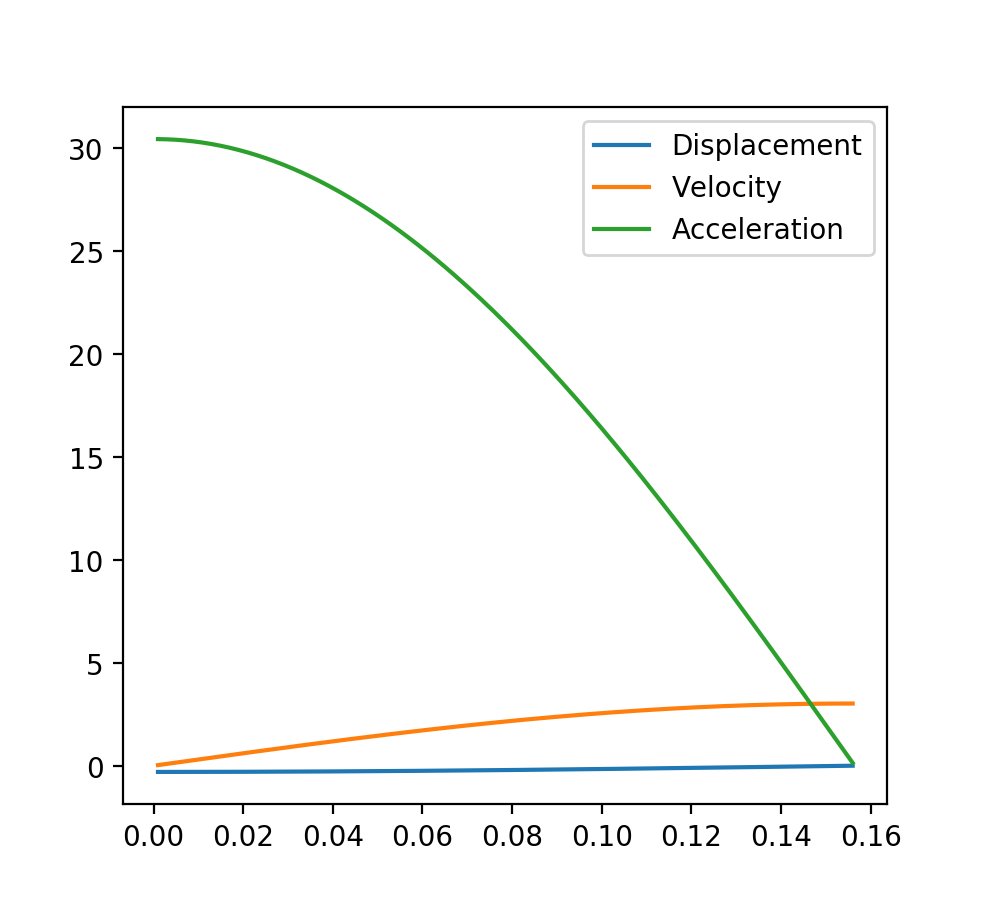
\includegraphics[width=\linewidth]{Hooke/hooke7000-0_3.png}
    \caption{Simulation to $x=0$}
    \label{fig:short}
  \end{subfigure}
  \begin{subfigure}[b]{.35\linewidth}
    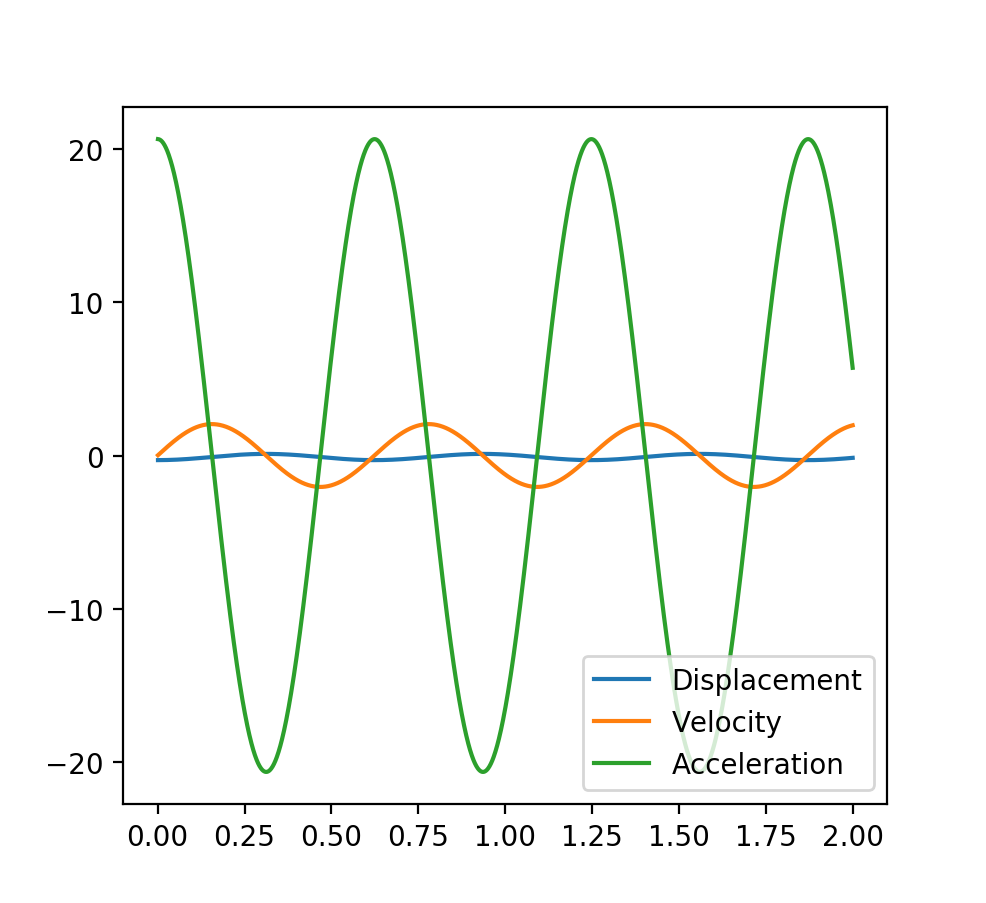
\includegraphics[width=\linewidth]{Hooke/hooke_shm.png}
    \caption{Simulation to $t=2$}
    \label{fig:shm}
  \end{subfigure}
\end{figure}

Given the parameters shown above, a mass of  69 kg, spring constant of 7000 N/m, and 
displacement of -.3 m, the robot would be launched 0.465 m, or around 18.3 inches, if vertical. Then, at an
angle of $50\degree$ the robot is able to fly 0.127 m vertically and .506 m horizontally. To find the lowest
spring constant, the spring constant would increase by some increment until the robot gets launched 0.33 m
vertically. The lowest spring constant candidate is $13120 \pm 10$ N/m and it would launch the robot .678 m
horizontally. Then to include a buffer, if the step height were 15 inches, or .38 m, the spring constant 
would need to be $14630 \pm 10$ N/m and it would travel .780 m horizontally.

For the possible mechanism, it would be best to have the longest throw as possible. When the displacement is
increased, but time to $x=0$ remains the same, Fig~\ref{fig:varyingDisplacement}. That means that the
overall power is more efficiently added by increasing the displacement. When the spring constant increases
the time decreases, but the force increases, shown in Fig~\ref{fig:varyingConstant}.

\begin{figure}[h]
  \caption{Varying Displacement}
  \label{fig:varyingDisplacement}
  \centering
  \begin{subfigure}[b]{.3\linewidth}
    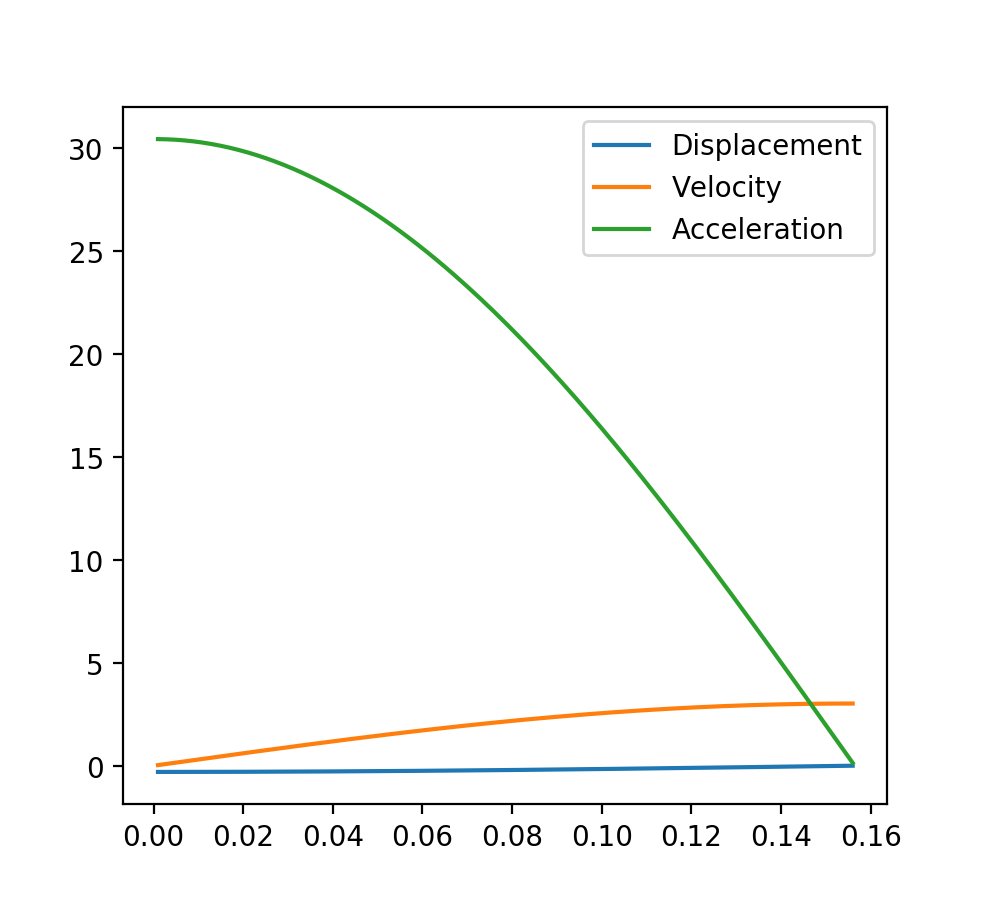
\includegraphics[width=\linewidth]{Hooke/hooke7000-0_3.png}
    \caption{$x=-0.3$}
  \end{subfigure}
  \begin{subfigure}[b]{.3\linewidth}
    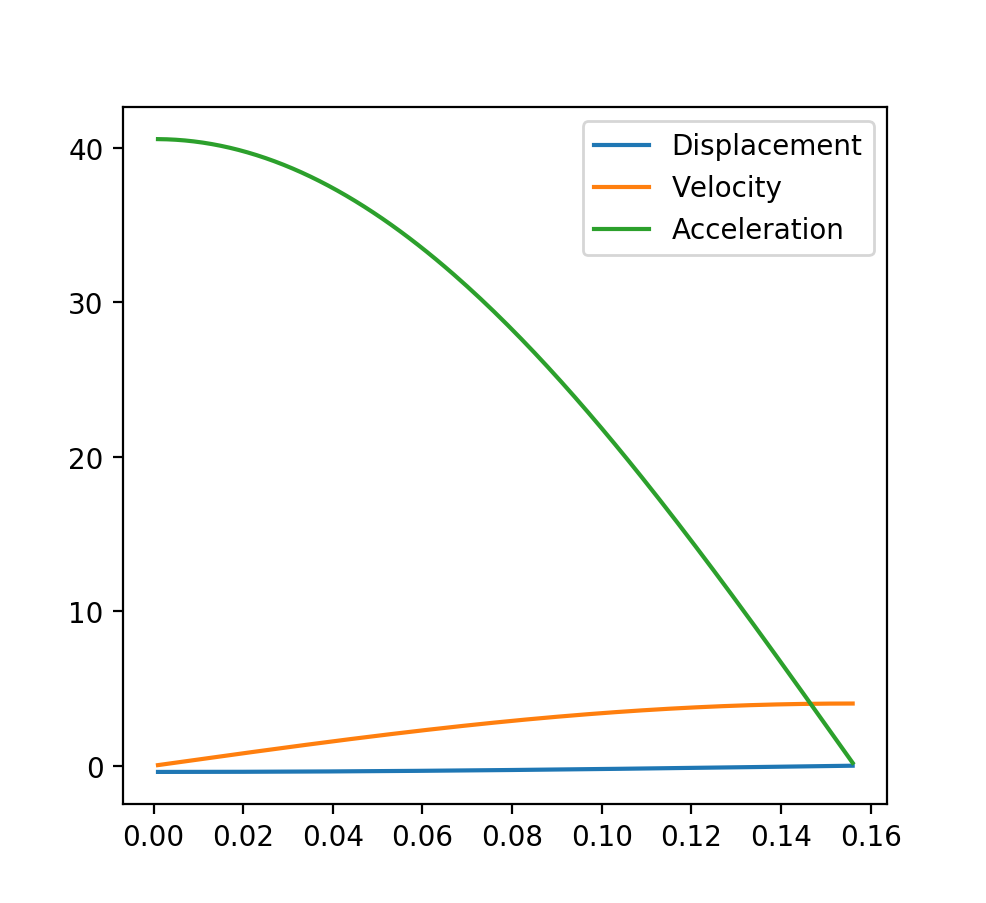
\includegraphics[width=\linewidth]{Hooke/hooke7000-0_4.png}
    \caption{$x=-0.4$}
  \end{subfigure}
  \begin{subfigure}[b]{.3\linewidth}
    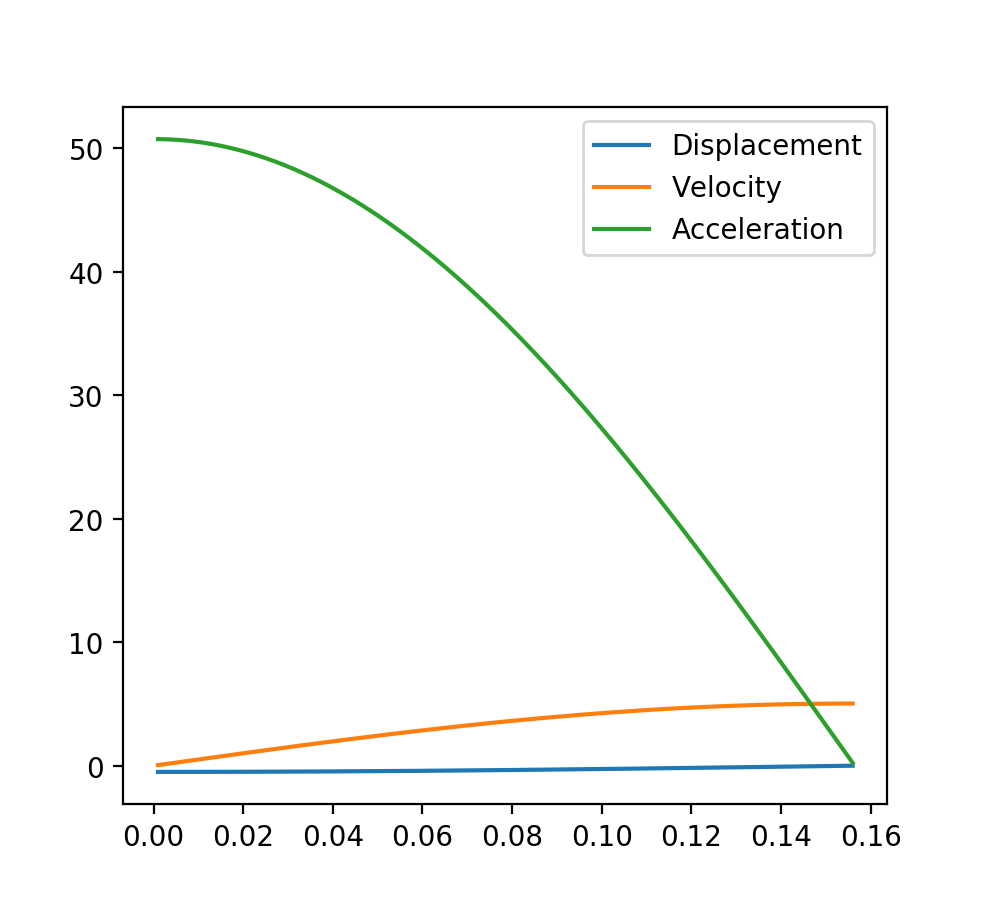
\includegraphics[width=\linewidth]{Hooke/hooke7000-0_5.png}
    \caption{$x=-0.5$}
  \end{subfigure}
\end{figure}

\begin{figure}[h]
  \caption{Varying Spring Constant}
  \label{fig:varyingConstant}
  \centering
  \begin{subfigure}[b]{.3\linewidth}
    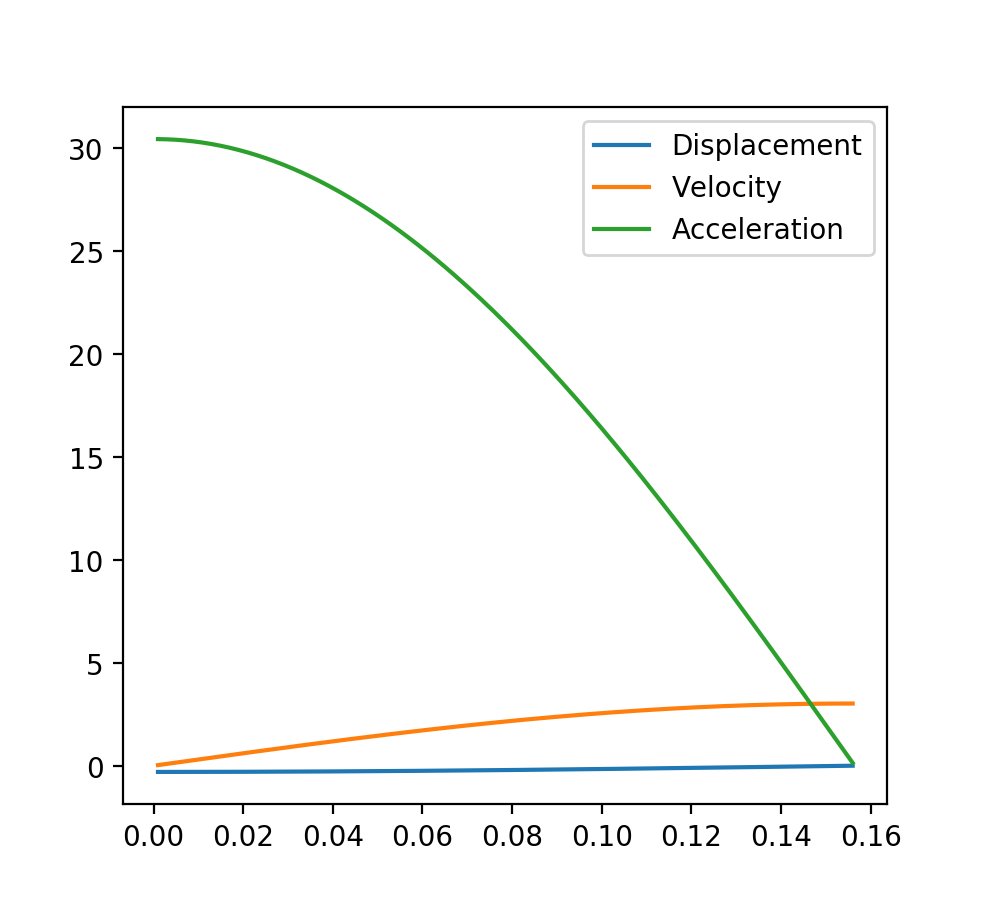
\includegraphics[width=\linewidth]{Hooke/hooke7000-0_3.png}
    \caption{$x=-0.3$}
  \end{subfigure}
  \begin{subfigure}[b]{.3\linewidth}
    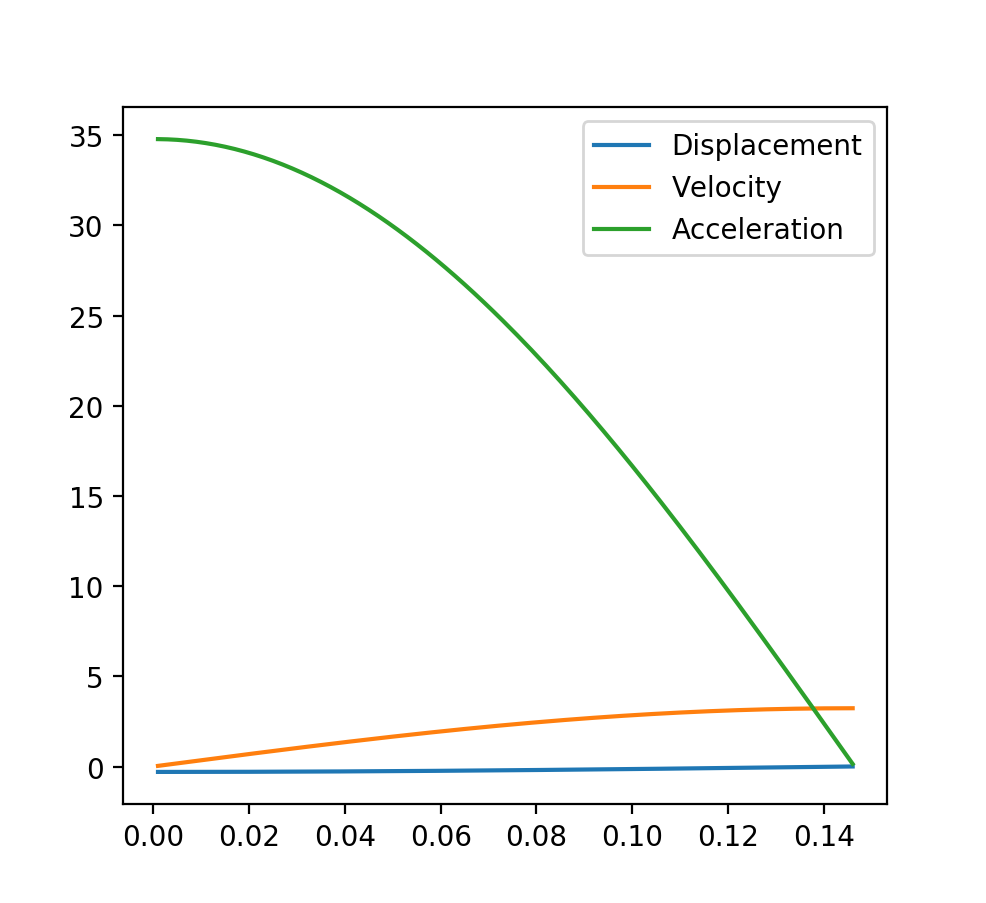
\includegraphics[width=\linewidth]{Hooke/hooke8000-0_3.png}
    \caption{$x=-0.4$}
  \end{subfigure}
  \begin{subfigure}[b]{.3\linewidth}
    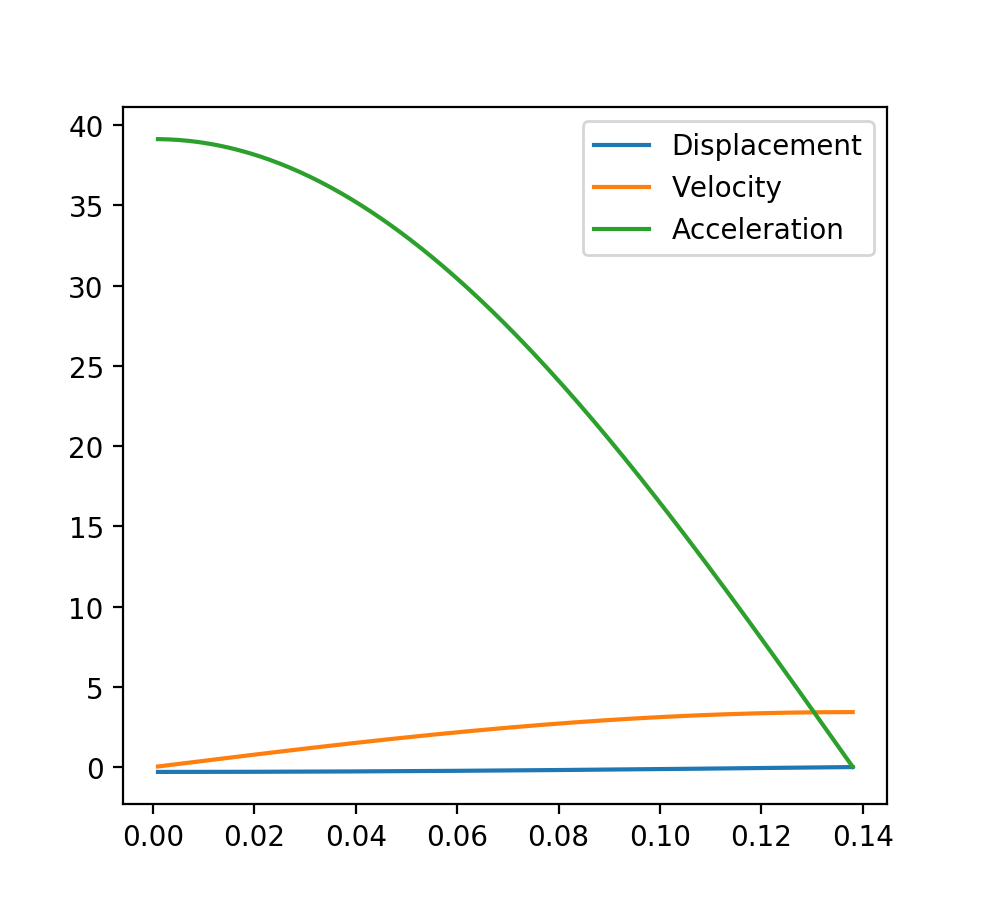
\includegraphics[width=\linewidth]{Hooke/hooke9000-0_3.png}
    \caption{$x=-0.5$}
  \end{subfigure}
\end{figure}

This result is intuitive especially when looking at real pogo sticks. They have relatively low weight springs
but they run the length of the stick, so they have a very long throw. The problem is that we would have at
most 18 inches of throw. The springs that can launch the robot given this relatively short displacement would
take up too much space to make sense.

\begin{figure}[h]
  \caption{Work given variables}
  \label{fig:workChanges}
  \centering
  \begin{subfigure}[b]{.45\linewidth}
    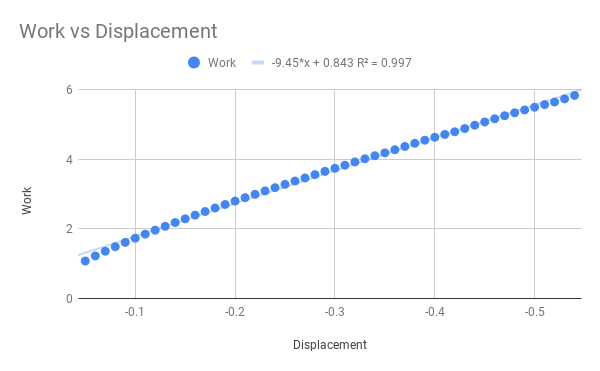
\includegraphics[width=\linewidth]{displacementRegress.png}
    \caption{Displacement}
  \end{subfigure}
  \begin{subfigure}[b]{.45\linewidth}
    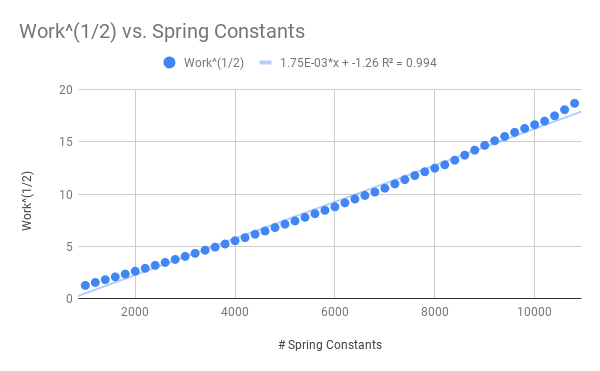
\includegraphics[width=\linewidth]{springRegress.png}
    \caption{Spring Constant}
  \end{subfigure}
\end{figure}
\newpage
Fig~\ref{fig:workChanges} shows the linear relationship between displacement and work done as well as between
the spring constant and the square root of the work. The $R^2$ value for the displacement is 0.997 showing a
clear linear relationship and the slope of -9.45 shows that displacement greatly affects the work. $R^2$ for
work is a little lower at .994, but still very linear. The more interesting number is the slope which is
$1.75*10^{-3}$ which shows that there is a weak connection between the spring constant and the work. This
analysis of Hooke's law backs up the engineering solution described earlier. Work was chosen for this
comparison since the important value is the total acceleration or force that is applied over the range of
motion. For the displacement calculations, the spring constant was held at 1000 N/m, and for the spring
constant calculations, the displacement was held at -.3 meters. The work was calculated by numerically
integrating the acceleration of the object times the mass times the change is position of velocity,
Equation(\ref{eq:workIntegral}).

\begin{singlespace}
\begin{equation}
  \label{eq:workIntegral}
  \int_{0}^{s} m a dx
\end{equation}
\begin{small}
  \begin{itemize}[label=]
    \item $s$: displacement
    \item $dx$: change in position or velocity
  \end{itemize}
\end{small}
\end{singlespace}

\section{Evaluation}
The accuracy and precision of this simulation could be improved. The model used is overly simplistic
since it does not take slippage on the ground, deviance from Hooke's law, friction, wear, and other
inefficiencies. Such inefficiencies would mean that this simulation overestimates the projectile motion. The
model presented to the team to prove if this mechanism was viable was the previously described system but
half of the force was lost to mechanical inefficiencies. Beyond an optimistic model, the numerical approach
for solving these equations yields, at least for me, a more intuitive way of describing the mechanics at the
cost of accuracy. The way to mitigate error would be to decrease the change in time, or increase the number
of iterations, which eventually accumulate significant floating point error. For computers, decimal numbers
are difficult to define and when doing successive operations on decimal numbers will eventually cause a small
error that propagates through the system. Because of this, computer simulations will never be perfect
representations of reality, but they can get very close.

This investigation also addresses major safety concerns. To actually test a mechanism of this sort would
require very large and stiff springs holding a lot of energy. Making a physical prototype of this design 
would be infeasible for a number of reasons: cost, time, and safety. There are also concerns about breaking
the field with this design. That means that this idea is dangerous due to the materials used, the tension of
the springs, and as well as the problems inherent in rapidly accelerating a 69 kg object.

\section{Conclusion}
The design proposed is preposterous. It is mathematically possible, but for all intents and purposes entirely
unfeasible. The power of the springs and their required range of motion would take up the majority of the
robots internal volume, and the tension these springs would be under would pose a major safety risk. Even if
we made this robot it would not be allowed to play.

\newpage{}
\printbibliography{}

\newpage{}
\section{Appendix}
\listoffigures{}


\begin{singlespace}
\subsection*{Pogo Equation Derivation}
\begin{equation}
  \label{eq:derivation}
  \begin{split}
    F &= ma \\
    F &= -kx \\
    \sum F &= -kx - mg\cos(\theta) \\
    ma &= -kx - mg\cos(\theta) \\
    m\ddot{x} &= -kx - mg\cos(\theta) \\
    m(\ddot{x} + g\cos(\theta)) &= -kx \\
    \ddot{x} + g\cos(\theta) &= \frac{-kx}{m} \\
    \ddot{x} &= \frac{-kx}{m} - g\cos(\theta)
  \end{split}
\end{equation}
\end{singlespace}

\section*{Code}
\lstinputlisting[language=Python, label={lst:springAcc}, caption={Spring Acceleration}]{code/spring.py}
\lstinputlisting[language=Python, label={lst:projForm}, caption={Formulatic Projectile Motion}]
{code/projectileFormulaic.py}
\lstinputlisting[language=Python, label={lst:pogo}, caption={Full Pogo Code}]{code/pogo.py}
\end{document}
